%%%%%%%%%%%%%%%%%%%%%%%%%%%%%%%%%%%%%%%%%%%%%%%%%%%%%%%%%%%%%%%%%%%%%%%%%%%%%%%%%%%%%%%%%%%%%%%%%%%%%%
%
%   Filename    : chapter_3.tex 
%
%   Description : This file will contain your Theoretical Framework.
%                 
%%%%%%%%%%%%%%%%%%%%%%%%%%%%%%%%%%%%%%%%%%%%%%%%%%%%%%%%%%%%%%%%%%%%%%%%%%%%%%%%%%%%%%%%%%%%%%%%%%%%%%

%\footnote{Oxford Dictionary. https://en.oxforddictionaries.com}
%\footnote{The Free Dictionary. http://www.thefreedictionary.com/}

\chapter{Theorerical Framework}
\label{sec:theoreticalframewrok}

This chapter introduces and expands on the relevant concepts and theories to be used over the course of this research.

%section~~~~~~~~~~~~~~~~~~~~~~~~~~~~~~~~~~~~~~~~~~~~~~~~~~~~~~~~~~~~~~
\section{Life Stories}
A \textit{life story}, or a biography, is an account of the series of events making up a person's life according to The Free Dictionary \footnote{The Free Dictionary. http://www.thefreedictionary.com/}. An \textit{autobiography}, or a \textit{memoir}, is an account of a person's life written by themselves according to Oxford Dictionary \footnote{Oxford Dictionary. https://en.oxforddictionaries.com}. An \textit{event} is anything that happens, especially one of importance according to Oxfor Dictionary \footnote{Oxford Dictionary. https://en.oxforddictionaries.com}.

The following sections describe the different elements of a story, and the linguistic concerns surrounding the expression of these elements. 

\subsection{Elements and Structure of a Story}
A story has a beginning, middle, and end portion (Pacis, personal communication, October 12, 2016). Failure to provide any of these parts renders a story incomplete and disinteresting. The linear structure of a story, as shown in \figref{fig:linearstructure}, is taken from (Pacis \& Gojo-Cruz, as cited by \cite{Chua2016}) as well as from (Hancock, 1994 as cited in Types of Plot, 2010), who states that a plot is a ``sequence of events that occurs to characters in situations in the beginning, middle, and end of a story.''

\begin{figure}[!htb]                %-- use [t] to place figure at top, [b] to place at the bottom, [h] for here
   \centering                    %-- use this to center the figure
   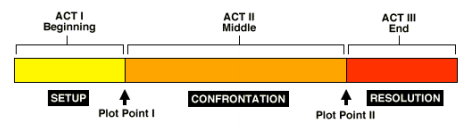
\includegraphics [width=\textwidth] {linearstructure.png}      %-- include image file named as "disneychart.png" 
   \caption{A model of the linear structure of a story.}
    \label{fig:linearstructure}
\end{figure}

As seen in \figref{fig:linearstructure}, events, details, or plot points, may occur that separate the beginning from the middle, and the middle from the end. 

\begin{figure}[!htb]                %-- use [t] to place figure at top, [b] to place at the bottom, [h] for here
   \centering                    %-- use this to center the figure
   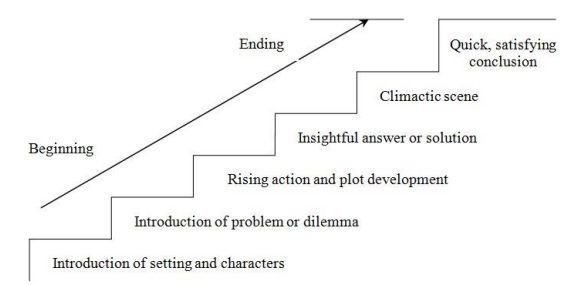
\includegraphics [width=\textwidth] {storystructure.png}      %-- include image file named as "disneychart.png" 
   \caption{The story structure used in Picture Books, which tells the (fictional) story of a child who is disobedient.}
    \label{fig:storystructure}
\end{figure}

Stories for children, such as those generated by the Picture Books story generation system \cite{SolisSiyTabiraoOng2009}, follow the structure of Machado (2003, as cited in \cite{SolisSiyTabiraoOng2009}) which consists of the introduction; a problem; rising action; solution; and climax. \figref{fig:storystructure} illustrates the structure of Picture Books 1's stories.

Some of the elements present in Picture Books' stories are only necessary in the case of fictional stories, while some will still be necessary, such as having a beginning and an end. Life stories, which are a different type of story from children's stories or other fictional stories, follow a different pattern. According to Youse \citeyear{Youse2005}, there are ten (10) necessary elements present in a life story. These are:
\begin{enumerate}
\item \textbf{Birthday and birthplace}. The story should be able to indicate when and where a person's life started.
\item \textbf{Family members}. Was this person the eldest in a few children? Did he/she eventually take a spouse and sire any children? Did he/she have notable relatives?
\item \textbf{Childhood and education life}. Early achievements or stories that happened early on in this person's life may have had an impact later on in his/her life.
\item \textbf{Hobbies, interests, and notable activities}. This is present for the reader to be able to get an initial impression of this person. Do the person's hobbies or activities make them more interesting? Do they relate to other aspects of their life? Being able to craft interesting stories is important in this research, and describing a person's hobbies is one part of it.
\item \textbf{Photos or likenesses}. Providing a likeness of the person will complete the impression the reader has about that person.
\item \textbf{Anecdotes}. Interesting stories about this person as told by others, that makes this person more interesting.
\item \textbf{Career} (if the person is old enough to have had one). Is their work a big reason on why a story is being told about them? Does their career relate to their interests, or past experiences? Did they make significant contributions to mankind by doing their job?
\item \textbf{Reason for fame}. At what point in their life did this person become noteworthy or famous, and why?
\item \textbf{Later life} (if the person is deceased). Did they continue their work and/or contributions to mankind later on in their life? Were they honored for their achievements?
\item \textbf{Death} (if the person is deceased). When and where did they die, and under what circumstance? Was there anything unusual or significant about their death? For example, U.S. Presidents Thomas Jefferson and John Adams both died on 4 July 1826; 4 July being the American Independence Day.
\end{enumerate}

All, or most of, these elements should be present in a life story. Such a story structure can be found by perusing articles about a person's life (e.g. Miriam Defensor Santiago). However, some elements (such as numbers 7-10 in the list above) are not possible to put into a person's life story because they may not be old enough. For these ones, concern should be put into ensuring that the story ends in a satisfying manner despite the missing details.

%section~~~~~~~~~~~~~~~~~~~~~~~~~~~~~~~~~~~~~~~~~~~~~~~~~~~~~~~~~~~~~~
\section{Facebook}

\subsection{Facebook Content}
Facebook contains a lot of data ranging from texts to photos and to videos. It contains numerous of varying stories, facts and events from users all around the world. Each user has the ability to post any content they prefer to which can be categorized into 13 categories, as shown in \figref{fig:facebookcontent}.

\begin{figure}[!htb]                %-- use [t] to place figure at top, [b] to place at the bottom, [h] for here
   \centering                    %-- use this to center the figure
   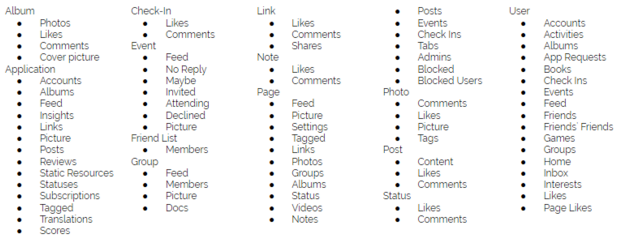
\includegraphics [width=\textwidth] {facebookcontent.png}      %-- include image file named as "disneychart.png" 
   \caption{Facebook content categorized into 13 categories.}
    \label{fig:facebookcontent}
\end{figure}

\subsection{Facebook Components}
Facebook is comprised of eight different components namely: [1] News Feed, [2] Friends, [3] Timeline, [4] Likes, Comments, and Shares, [5] Messages and Inbox, [6] Notifications, [7] Groups and [8] Statuses or Posts. In this section, only the status or posts component will be discussed since these will be the focus of the research.

\subsubsection{Status or Posts}
In 2013, Facebook has added a new structured status update feature allowing users to specify what they are feeling, watching, listening, playing, celebrating, among others \cite{darwell}. Those which we will be using for event classification in this research are the following:

\begin{enumerate} [label=\alph*.]
\item Celebrating - Shows what the user is remembering at the time of posting.
\item Travelling To - Tells where the user is travelling at the time of the status update. The user can include the Facebook page of the location he/she is currently travelling to or he/she can simply include the location if there is no Facebook page for that.
\item Eating - Tells what food the user is consuming.
\item Drinking - Tells what beverage the user is drinking.
\end{enumerate}

%section~~~~~~~~~~~~~~~~~~~~~~~~~~~~~~~~~~~~~~~~~~~~~~~~~~~~~~~~~~~~~~
\section{Data Extraction Tool}
For this research, Graph API was used for data extraction. Graph API is a low-level HTTP-based API that is primarily used to access data and information in Facebook's platform \cite{FacebookGraphAndroid2016}. It allows applications to do certain actions in Facebook such as publish updates, media files and even schedule a post. 

\subsection{Structure}
The structure of Graph API consists of three main types, namely: nodes, edges and fields. Nodes are the basic components of Facebook such as a user, page, or comment; edges are the connections between the nodes, such as the connection between a user's photo and that photo's comment; and fields are the details or information about a specific node, such as the first and last names of the user.

These nodes can be accessed through making HTTP GET requests passed to the API at graph.facebook.com or graph-video.facebook.com for video uploads. Most APIs would require access tokens which determine the permissions for secure access to Facebook APIs. Each access token contains information about the token's expiration as well as the application in which it was generated (in this case, our system).

When a user logs into Facebook through an application (or app), the app will be able to obtain an access token which allows access to the user's data on Facebook \cite{FacebookToken2013}. Logging in only accesses the basic permissions such as the public default. Additional permissions can be listed down in the scope parameter and would inform whether the user would choose to authenticate the app with the said permissions \cite{FacebookJavaScript}. The user access tokens are then automatically stored by the Facebook SDK for JavaScript. These can be retrieved through FB.getAuthResponse which obtains the access token within the received response.

\subsection{JSON File}
Once the access token with the prefered permissions is obtained, the system can access the user's Facebook data through HTTP GET requests and receive a JSON file containing the requested information from the user.  The structure of the JSON file received may vary depending on the node or edges read \cite{FacebookGraphAndroid2016}. The general form for this is:
	\{
		 ``fieldname'' : \{field-value\}, ….
	\}
	
%section~~~~~~~~~~~~~~~~~~~~~~~~~~~~~~~~~~~~~~~~~~~~~~~~~~~~~~~~~~~~~~
\section{Text Understanding}
For this research, the Stanford CoreNLP API, a service that gives access to a set of natural language analysis tools, was used. More specifically, the API's part-of-speech tagger, named entity recognizer, parser, and universerval dependencies were used to understand text. The API takes in a string as an input and its output can be viewed in four different ways, each of which was shown by the aforementioned tools.

Given the sentence, ``Robee is a 4th year student of De La Salle University taking up Bachelor of Science in Computer Science.", the API produces the results shown in \figref{fig:stanford-aner}, \figref{fig:stanford-parsingsample}, \figref{fig:stanford-parsetree2}, and \figref{fig:stanford-dependencies2}, for named entity recognition, part-of-speech tagging, parsing, and universal dependencies.

\subsection{Named Entity Recognition}
Named Entity Recognition (NER) is a process that classifies entities in the given text and categorizes them as person, organization, location, among other classifiers. The Stanford CoreNLP API determines the known entities and returns information about those entities. 

In the CoreNLP package, it has two classes, Annotation, and Annotator. Annotations are data structures that hold the results put out by Annotators. They can hold parsed data, part-of-speech tags, or named entity tags. Annotators, on the other hand, work like functions. They can parse and tokenize text and perform NER tagging on sentences. Annotations and Annotators are integrated by AnnotationPipelines, which can create sequences of Annotators. 

To construct a Stanford CoreNLP object from a given set of properties, StanfordCoreNLP (Properties props) must be used. The method creates a pipeline using the given annotators in the annotators property.

\begin{figure}[!htb]                %-- use [t] to place figure at top, [b] to place at the bottom, [h] for here
	\centering                    %-- use this to center the figure
	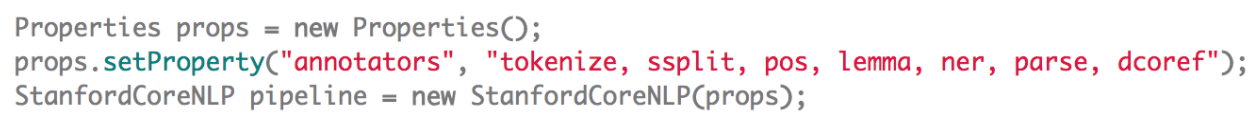
\includegraphics [width=\textwidth] {stanford-pipeline.png}      %-- include image file named as "disneychart.png" 
	\caption{Sample Code for Creating Pipeline}
	\label{fig:stanford-pipeline}
\end{figure}

The code snippet shown in \figref{fig:stanford-pipeline} creates a Stanford CoreNLP object with the following annotators: named entity recognition, part-of-speech tagging, parsing, and lemmatization. For named entity recognition, the ner annotator is used.

\begin{figure}[!htb]                %-- use [t] to place figure at top, [b] to place at the bottom, [h] for here
	\centering                    %-- use this to center the figure
	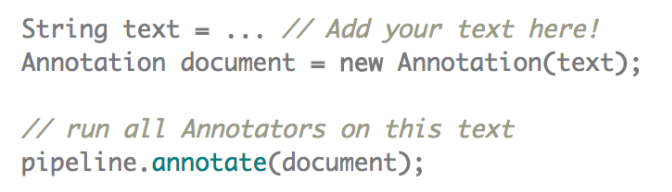
\includegraphics [width=\textwidth] {stanford-parsing.png}      %-- include image file named as "disneychart.png" 
	\caption{Sample Code for Parsing Text}
	\label{fig:stanford-parsing}
\end{figure}

After creating a Stanford CoreNLP object, the annotate(Annotation document) method is used to parse arbitrary text as shown in \figref{fig:stanford-parsing}. 

\begin{figure}[!htb]                %-- use [t] to place figure at top, [b] to place at the bottom, [h] for here
	\centering                    %-- use this to center the figure
	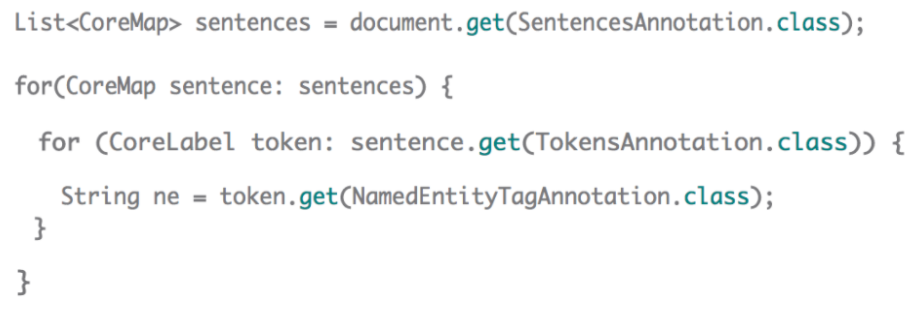
\includegraphics [width=\textwidth] {stanford-ner.png}      %-- include image file named as "disneychart.png" 
	\caption{Sample Code for Named Entity Recognition}
	\label{fig:stanford-ner}
\end{figure}

The output of the Annotators is accessed using the data structures CoreMap and CoreLabel (in \figref{fig:stanford-ner}). Entity type for each token can be retrieved using the get (NamedEntityTagAnnotation.class). 

The analysis of the online version of Stanford CoreNLP from the sample input returned a set of detected entities namely, ``Robee" and ``De La Salle University"; along with their corresponding types (shown in \figref{fig:stanford-aner}).

\begin{figure}[!htb]                %-- use [t] to place figure at top, [b] to place at the bottom, [h] for here
	\centering                    %-- use this to center the figure
	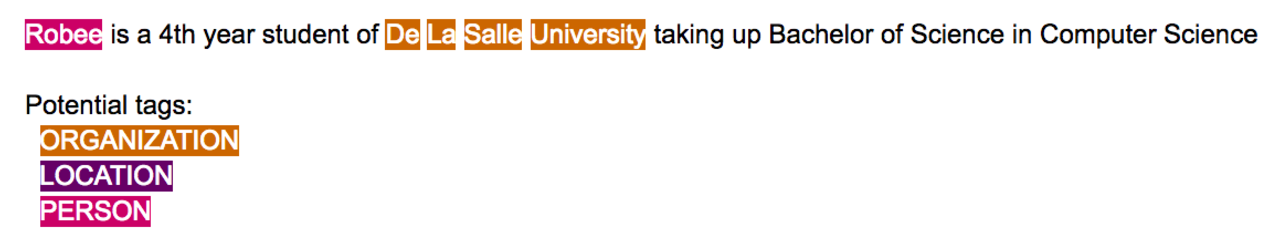
\includegraphics [width=\textwidth] {stanford-aner.png}      %-- include image file named as "disneychart.png" 
	\caption{Actual Named Entity Recognition Output by Stanford CoreNLP}
	\label{fig:stanford-aner}
\end{figure}

\subsection{Part-of-Speech Tagging}
A Part-of-Speech Tagger is a piece of software that can read text in some language, break it down into tokens, and assign a part to each token, such as \textit{noun}, \textit{verb}, or \textit{adjective}. 

For the part-of-speech tagging, the pos annotator is used to label tokens with their POS tag. 

\begin{figure}[!htb]                %-- use [t] to place figure at top, [b] to place at the bottom, [h] for here
	\centering                    %-- use this to center the figure
	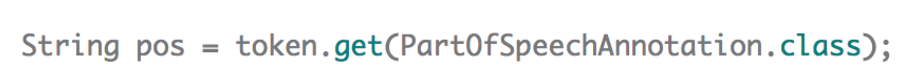
\includegraphics [width=\textwidth] {stanford-parsing-token.png}      %-- include image file named as "disneychart.png" 
	\caption{Sample Code for Getting the Part-of-Speech Tag of Each Token}
	\label{fig:stanford-parsingtoken}
\end{figure}

Part-of-speech tag of each token can be retrieved using the get(PartOfSpeechAnnotation.class) method shown in \figref{fig:stanford-parsingtoken}. A sample part-of-speech tagging using the online version of Stanford CoreNLP is shown in \figref{fig:stanford-parsingsample}.

\begin{figure}[!htb]                %-- use [t] to place figure at top, [b] to place at the bottom, [h] for here
	\centering                    %-- use this to center the figure
	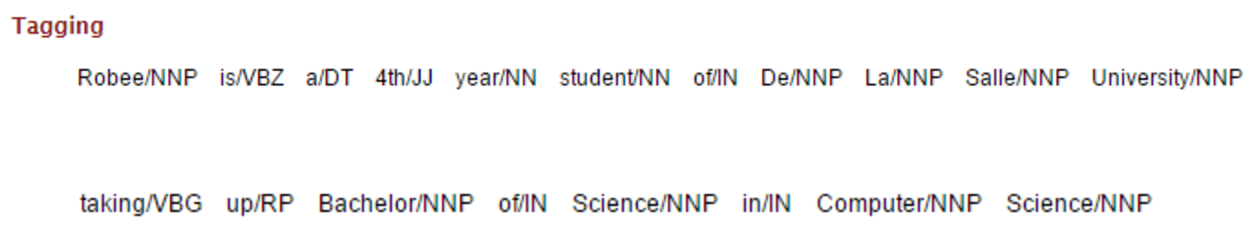
\includegraphics [width=\textwidth] {stanford-parsingsample.png}      %-- include image file named as "disneychart.png" 
	\caption{Sample Part-of-speech Tagging using Stanford CoreNLP}
	\label{fig:stanford-parsingsample}
\end{figure}

\subsection{Parsing}
The \textit{parser} annotator generates the parse tree for each sentence. It mainly analyzes the grammatical structure of sentences, for instance, determining which set of words are of the same group and which words are the subject, doer, or receiver of the action.

The sample parser returned by the online version of Stanford CoreNLP from the input is shown in \figref{fig:stanford-parsetree2}.

\begin{figure}[!htb]                %-- use [t] to place figure at top, [b] to place at the bottom, [h] for here
	\centering                    %-- use this to center the figure
	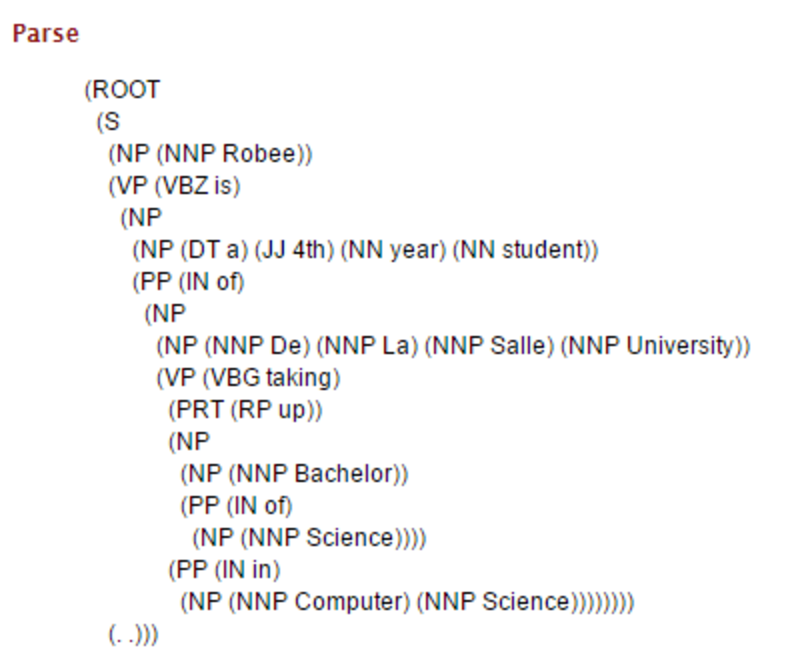
\includegraphics [width=\textwidth] {stanford-parsetree2.png}      %-- include image file named as "disneychart.png" 
	\caption{Parse Tree Output by Stanford CoreNLP}
	\label{fig:stanford-parsetree2}
\end{figure}

\clearpage
\subsection{Universal Dependencies}
The Universal Dependencies annotator generates all the possible relationships of one token to the other tokens. It mainly does the full syntactic analysis of the sentence and checks which tokens has a relationship with the others based on the probabilistic parser \cite{Manning14thestanford}. 

An example of the universal dependencies returned by the online version of Stanford CoreNLP from the input is shown in \figref{fig:stanford-dependencies2}.

\begin{figure}[!htb]                %-- use [t] to place figure at top, [b] to place at the bottom, [h] for here
	\centering                    %-- use this to center the figure
	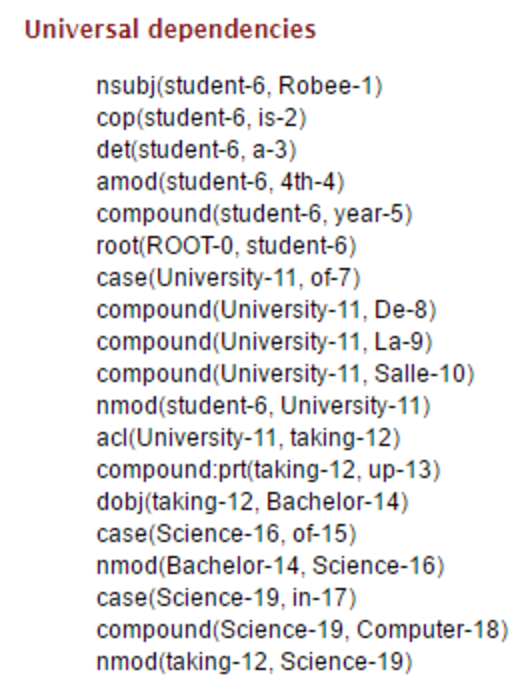
\includegraphics  [width=4in,height=6in,keepaspectratio] {stanford-dependencies2.png}      %-- include image file named as "disneychart.png" 
	\caption{Universal Dependencies Output by Stanford CoreNLP}
	\label{fig:stanford-dependencies2}
\end{figure}

\clearpage
%section~~~~~~~~~~~~~~~~~~~~~~~~~~~~~~~~~~~~~~~~~~~~~~~~~~~~~~~~~~~~~~
\section{Text Generation}
Natural language generation (NLG) is defined as the process of constructing thoughts or non-linguistic inputs into understandable English texts \cite{IndurkhyaDamerau2010, JurafskyMartin2000, ReiterDale1997}. It uses concepts stored in a knowledge base and decides how to generate text that humans can understand.

An NLG system's task is described as mapping the input data to an output text \cite{ReiterDale1997}. An NLG system must perform six different tasks that needs to be done in order to produce a final output text from the given input. The process in each task is discussed below.

\subsection{Content Determination}
During content determination, the NLG system decides what information needs to be communicated in the text from the given input \cite{ReiterDale1997}. Content must be appropriate for the reader or the user \cite{JurafskyMartin2000}. This process will create messages from the knowledge base. These messages are represented as data objects and will be passed to the next process. The whole message creation process is consists of filtering and summarizing the input data and the messages created can be expressed as entities, concepts and relations in the domain \cite{ReiterDale1997}. In \figref{fig:ContentDeterminition}, three different messages are created.

\clearpage
\begin{figure}[!htb]                %-- use [t] to place figure at top, [b] to place at the bottom, [h] for here
   \centering                    %-- use this to center the figure
   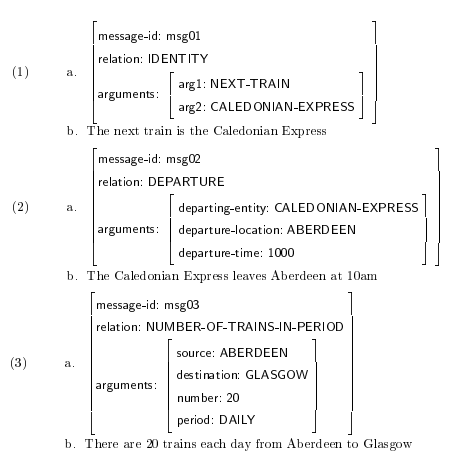
\includegraphics [width=4in,height=4in,keepaspectratio] {ContentDeterminition.png}      %-- include image file named as "disneychart.png" 
   \caption{Sample Messages} \cite{ReiterDale1997}
    \label{fig:ContentDeterminition}
\end{figure}

\subsection{Discourse Planning}
In comparison to stories having a beginning, middle and end, a message must have a structure, one which must be logical and more distinguishable than the structure used for stories\cite{ReiterDale1997}. In the process of discourse planning, the ordering and structuring of the messages produced by the content determination are done. Content determination has no knowledge of the discourse structure which the message resides nor the content of the message itself \cite{JurafskyMartin2000}.

In generating stories, the system needs to produce a multi-message output. The easiest way is to produce a message for each intended meaning, but what most cases require is the structuring of messages in an appropriate way \cite{JurafskyMartin2000}. For example: ``I have just compiled a simple C program. I have just run a single C program. The environment is configured properly.'' These three messages are individually coherent but are not joined properly.

The discourse planning process results in a tree structure. The leaf nodes represents the individual messages and the internal nodes tells how these messages are placed together and how they are related to one another. Sometimes, the internal nodes also include the discourse relations between their children. For example, as seen in \figref{fig:TreeStructureDiscoursePlanning}, the leaf node [DEPARTURE] is an elaboration of the leaf node [IDENTITY]. Later, these clusterings will have an impact in the determination of the sentence and paragraph boundaries of the final output.

\begin{figure}[!htb]                %-- use [t] to place figure at top, [b] to place at the bottom, [h] for here
   \centering                    %-- use this to center the figure
   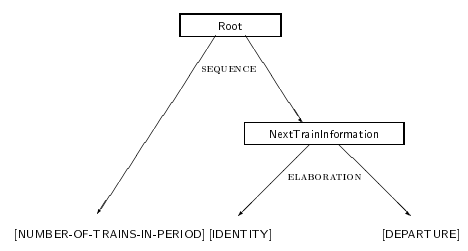
\includegraphics [width=4in,height=4in,keepaspectratio] {TreeStructureDiscoursePlanning.png}      %-- include image file named as "disneychart.png" 
   \caption{Tree Structure Returned by the Discourse Planning} \cite{ReiterDale1997}
    \label{fig:TreeStructureDiscoursePlanning}
\end{figure}

The discourse planner is composed of two main components for building the discourse structure namely: (1) Text Schemata and (2) Rhetorical Relations. 

\subsubsection{Text Schemata}
A simple method of generating text is positioning words into the templates. Another way to generate texts is to make choices based on the stored data according to the matched patterns in the system's knowledge base \cite{IndurkhyaDamerau2010}.

An observation of using the text schemata is that the texts follow a structural pattern. The schemata is represented by an augmented transition network (ATN) as shown in \figref{fig:AugmentedTransitionNetwork} which consists of states that is represented by an information that is chosen from the collection of data and transitions from one state to the other \cite{JurafskyMartin2000, IndurkhyaDamerau2010}. The transition between the states can be described as the cause followed by the effect, a sequence of events, and so on. State S0 defines the start state and State S2 defines the goal state. A loop in the states tells that there are additional information about the object, and sub-steps or side-effects of an action. 

\clearpage
\begin{figure}[!htb]                %-- use [t] to place figure at top, [b] to place at the bottom, [h] for here
   \centering                    %-- use this to center the figure
   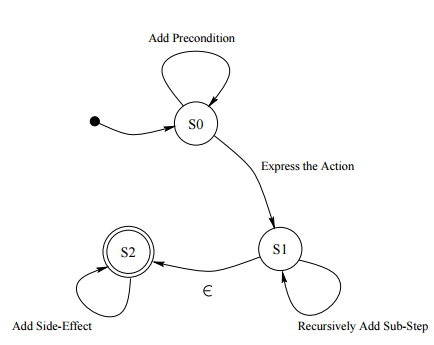
\includegraphics [width=4in,height=4in,keepaspectratio] {AugmentedTransitionNetwork.png}      %-- include image file named as "disneychart.png" 
   \caption{Augmented Transition Network (ATN)} \cite{JurafskyMartin2000}
    \label{fig:AugmentedTransitionNetwork}
\end{figure}

Using the text schemata is more flexible than directly placing words into the templates. The output was structured according to patterns of expression and add other informations extracted from the knowledge base \cite{JurafskyMartin2000}.

\subsubsection{Rhetorical Relations}
Rhetorical Structure Theory (RST), is a descriptive theory of text organization based on the relationships of two or more messages (Mann and Thompson, 1987 as cited in \cite{JurafskyMartin2000}). Some of the common RST relations are as follow \cite{JurafskyMartin2000}:
\begin{enumerate}
\item ELABORATION - This shows additional details about the content of the message. Elaboration may be in a form of:  (1) a member of a set, (2) an instance of an abstract class, (3) a part of a whole, (4) a step of a process, (5) an attribute of an object, and (6) a specific instance of a generalization.
\item CONTRAST - This shows things that, while there are some similarities between the two messages, they are still different in some other ways.
\item CONDITION - This states that something must happen in one of the messages before the situation in the other message can happen.
\item PURPOSE - One of the messages contains the goal of the other message.
\item SEQUENCE - The messages are in arranged in a sequence.
\item RESULT - One of the two messages is an outcome of the other message.
\end{enumerate}

\subsection{Sentence Aggregation}
This process organizes messages together into sentences. Based from the tree output of the Discourse Planning, the leaf nodes [IDENTITY] and [DEPARTURE] are together, so the sentence aggregation can combine the two messages into a single sentence which can be aggregated as ``The next train, which leaves at 10am, is the Caledonian Express.''. Sentence aggregation is not always required. Some of the messages can be expressed as a single sentence, but it would not result to the readability of the text \cite{ReiterDale1997}.

\subsection{Lexicalization}
In this process, the system maps the right words and phrases to convey the concepts and relations of the messages. The problem in lexicalization is the choosing of appropriate words or phrases to express the content \cite{JurafskyMartin2000}. For example, the words ``leave'' and' ``depart'' are both associated with the word ``derapture'' and the lexical selection must only choose one word to associate departure. Sometimes, lexicalization are simplified by hard-coding a single term with each entry in the knowledge base \cite{JurafskyMartin2000}. Although, this could be improved by varying the words used to express the concept or relation to obtain variety \cite{ReiterDale1997}. 

\subsection{Referring Expression Generation}
The task of creating referring expressions to identify the entities are done by the referring expression generation (REG). The Referring Expression (RE) is any noun phrase, whose task is to give identification to the objects (persons, things, or events). REG's goal is to add information to identify the entities unambiguously \cite{ReiterDale1997}. For example, in the sentence: ``The next train is the \textit{Caledonian Express. It} leaves at 10am. Many tourist guidebooks highly recommend \textit{this train}.'', the entity [CALEDONIAN-EXPRESS] from the content determination is referred to the ``Caledonian Express''; the second time to express Caledonian express is written as the pronoun ``it'' and  the use of ``this train'' to refer something that was already introduced before. REG and lexicalization are closely associated since both process chooses words and phrases to associated the domain. However, the referring expression generation needs to gather previous information to differentiate one entry from other entries. 

\subsection{Linguistic Realization}
Reiter \& Dale \citeyear{ReiterDale1997} explained the last process as applying grammar rules in order to generate a text which is syntactically, morphologically and orthographically correct. The sentence generated is syntactically correct when the grammatical arrangement of words in the sentence is correct; morphologically correct when the structure and form of words are correct; and orthographically correct when the words have correct spelling, hyphenation, capitalization, and punctuation. For example, in the sentence ``There are 20 trains each day from Aberdeen to Glasgow'', (1) the syntactic component of the linguistic realizer added the function words ``from'' and ``to" to describe the train's source and destination, (2) the morphological component of the linguistic realiser converted ``train'' to its plural form ``trains'', and (3) the orthographical component of the linguistic realizer capitalized the first word of the sentence and added a period (.) at the end of the sentence \cite{ReiterDale1997}.

\subsection{SimpleNLG}
SimpleNLG, a Java API for Natural Language Generation, is used to help write a program that can generate grammatically correct English sentences.  

\begin{figure}[!htb]                %-- use [t] to place figure at top, [b] to place at the bottom, [h] for here
	\centering                    %-- use this to center the figure
	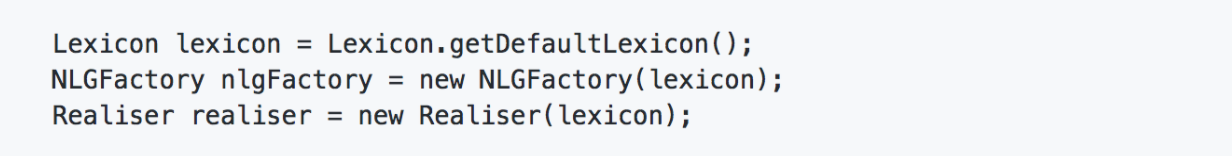
\includegraphics [width=4in,height=4in,keepaspectratio] {simplenlgA.png}      %-- include image file named as "disneychart.png" 
	\caption{SimpleNLG's lexicon, nlgFactory, and realiser}
	\label{fig:simplenlgA}
\end{figure}

Before the API can generate actual sentences, SimpleNLG lexicon, NLGFactory, and realiser are instantiated (shown in \figref{fig:simplenlgA}). Like any other natural language processing systems, SimpleNLG uses information about words from lexicons. SimpleNLG comes with a default lexicon that can be accessed via Lexicon lexicon = Lexicon.getDefaultLexicon(). NLGFactory is used to create SimpleNLG structures, and a realiser is used to transform SimpleNLG structures into text.

\begin{figure}[!htb]                %-- use [t] to place figure at top, [b] to place at the bottom, [h] for here
	\centering                    %-- use this to center the figure
	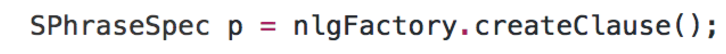
\includegraphics [width=4in,height=4in,keepaspectratio] {simplenlgB.png}      %-- include image file named as "disneychart.png" 
	\caption{SimpleNLG's SPhraseSpec} 
	\label{fig:simplenlgB}
\end{figure}

To generate sentences, a class called SPhraseSpec is used, which is accessible through the NLGFactory, using the createClause method (shown in \figref{fig:simplenlgB}). 

\begin{figure}[!htb]                %-- use [t] to place figure at top, [b] to place at the bottom, [h] for here
	\centering                    %-- use this to center the figure
	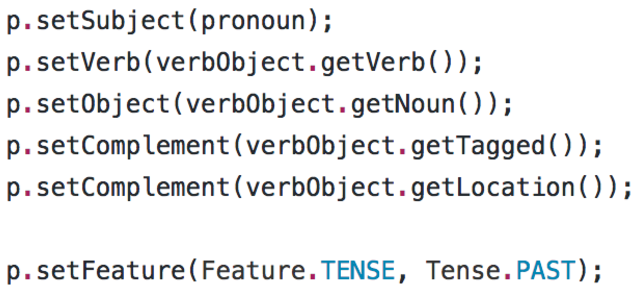
\includegraphics [width=4in,height=4in,keepaspectratio] {simplenlgC.png}      %-- include image file named as "disneychart.png" 
	\caption{SimpleNLG's SPhraseSpec methods}
	\label{fig:simplenlgC}
\end{figure}

SPhraseSpec allows for defining a sentence in terms of its syntactic constituents, which can be useful for specifying different parts of a sentence or clause, in no particular order. SimpleNLG then assembles those parts into grammatically correct sentences. The setSubject(subject), setVerb(verb), setObject(object), setComplement(complement), and setFeature(tense, tense) methods are used to define the sentence's subject, verb, object, complement, and tense respectively (shown in \figref{fig:simplenlgC}).

\begin{figure}[!htb]                %-- use [t] to place figure at top, [b] to place at the bottom, [h] for here
	\centering                    %-- use this to center the figure
	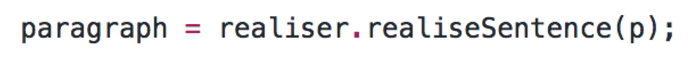
\includegraphics [width=4in,height=4in,keepaspectratio] {simplenlgD.png}      %-- include image file named as "disneychart.png" 
	\caption{SimpleNLG's realiser}
	\label{fig:simplenlgD}
\end{figure}

Given the subject - She; verb - going; object - to the mall; tagged - none; location - none; and verb tense - past. The realiser takes in the different components of the sentence, combines them, and generates a syntactically and morphologically correct text using the code snippet shown in \figref{fig:simplenlgD}.  The resulting sentence will then result to ``She went to the mall.”.

%section~~~~~~~~~~~~~~~~~~~~~~~~~~~~~~~~~~~~~~~~~~~~~~~~~~~~~~~~~~~~~~
\section{Knowledge Base}
This section discusses the different existing knowledge bases that were used in the implementation of the system: WordNet and ConceptNet.

\subsection{WordNet}
WordNet's database provides connections among nouns and verb synsets containing words that share an underlying meaning. It contains derivational links that connect noun and verb senses (e.g. travel - traveller). 

A singleton instance of Dictionary is used to query WordNet using JWNL (shown in \figref{fig:jwnl-instantiation}).

\begin{figure}[!htb]                %-- use [t] to place figure at top, [b] to place at the bottom, [h] for here
	\centering                    %-- use this to center the figure
	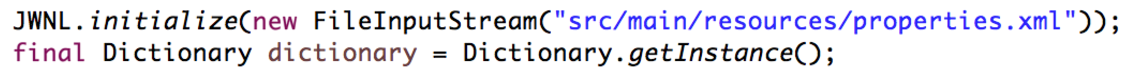
\includegraphics [width=4in,height=4in,keepaspectratio] {jwnl-instantiation.png}      %-- include image file named as "disneychart.png" 
	\caption{Instantiation of the Dictionary}
	\label{fig:jwnl-instantiation}
\end{figure}

Afterwards, a lemma can easily be queried from the dictionary (e.g. travel). For each lemma, there can be one part-of-speech specified among four possible part-of-speech classes: \textit{POS.ADJECTIVE}, \textit{POS.ADVERB}, \textit{POS.NOUN}, and \textit{POS.VERB}. 

The system checks if the lemma is in the dictionary. If the lookup fails, \textit{indexWord} is null as shown in \figref{fig:wn-indexword}.

\begin{figure}[!htb]                %-- use [t] to place figure at top, [b] to place at the bottom, [h] for here
	\centering                    %-- use this to center the figure
	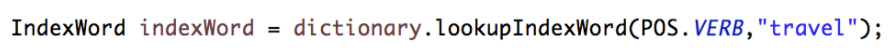
\includegraphics [width=4in,height=4in,keepaspectratio] {wn-indexword.png}      %-- include image file named as "disneychart.png" 
	\caption{Setting the lemma and part of speech}
	\label{fig:wn-indexword}
\end{figure}

Different senses that the lemma may have are retrieved as shown in Figure \figref{fig:wn-senses}.

\begin{figure}[!htb]                %-- use [t] to place figure at top, [b] to place at the bottom, [h] for here
	\centering                    %-- use this to center the figure
	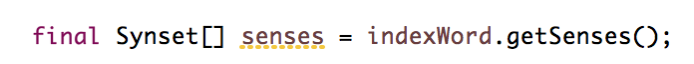
\includegraphics [width=4in,height=4in,keepaspectratio] {wn-senses.png}      %-- include image file named as "disneychart.png" 
	\caption{Getting related senses}
	\label{fig:wn-senses}
\end{figure}

For each sense, a short description of the sense called \textit{gloss} is derived as shown in \figref{fig:wn-gloss}. 

\begin{figure}[!htb]                %-- use [t] to place figure at top, [b] to place at the bottom, [h] for here
	\centering                    %-- use this to center the figure
	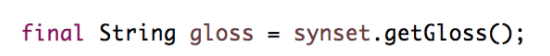
\includegraphics [width=4in,height=4in,keepaspectratio] {wn-gloss.png}      %-- include image file named as "disneychart.png" 
	\caption{Getting short description of senses}
	\label{fig:wn-gloss}
\end{figure}

Other more specific lemmas under each sense are also derived as shown in \figref{fig:wn-words}. 

\begin{figure}[!htb]                %-- use [t] to place figure at top, [b] to place at the bottom, [h] for here
	\centering                    %-- use this to center the figure
	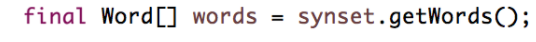
\includegraphics [width=4in,height=4in,keepaspectratio] {wn-words.png}      %-- include image file named as "disneychart.png" 
	\caption{Getting words under specific senses}
	\label{fig:wn-words}
\end{figure}

WordNet returns senses containing related lemmas as shown in \figref{fig:wn-output}.

\begin{figure}[!htb]                %-- use [t] to place figure at top, [b] to place at the bottom, [h] for here
	\centering                    %-- use this to center the figure
	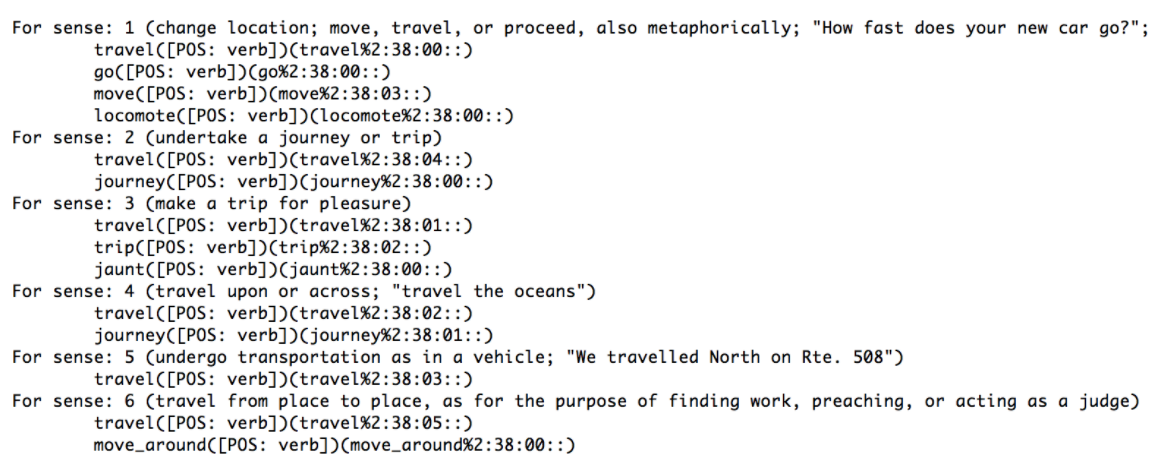
\includegraphics [width=4in,height=4in,keepaspectratio] {wn-output.png}      %-- include image file named as "disneychart.png" 
	\caption{Related senses returned by WordNet}
	\label{fig:wn-output}
\end{figure}

By using the mapping available on WordNet's database, morphosemantically-related words are extracted as shown in \figref{fig:wn-output2}.

\begin{figure}[!htb]                %-- use [t] to place figure at top, [b] to place at the bottom, [h] for here
	\centering                    %-- use this to center the figure
	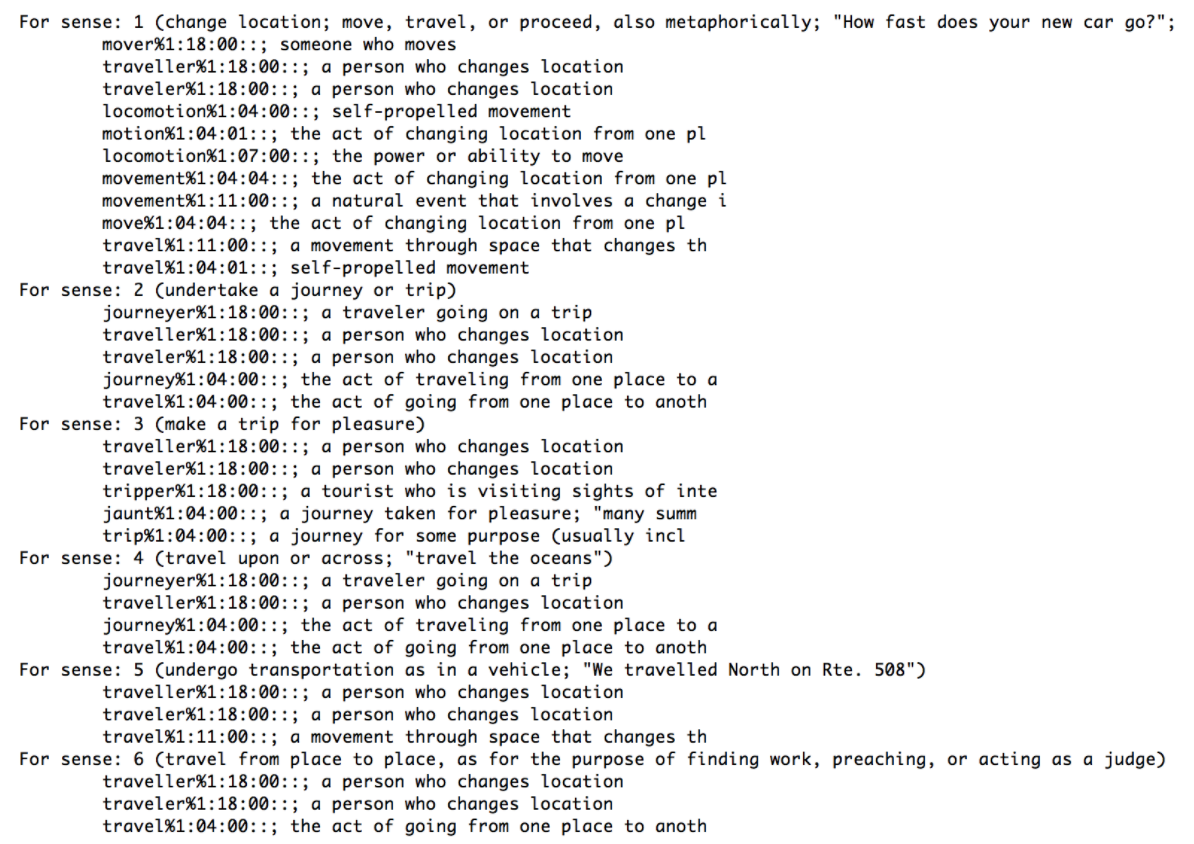
\includegraphics [width=4in,height=4in,keepaspectratio] {wn-output2.png}      %-- include image file named as "disneychart.png" 
	\caption{Morphosemantically related words returned by WordNet}
	\label{fig:wn-output2}
\end{figure}

\subsection{ConceptNet}
ConceptNet is a semantic network containing nodes or concepts which are represented by words or short phrases (e.g. ``ball'', ``toy'') and the semantic relations between them (e.g. ``IsA'', ``PropertyOf'') \footnote{http://conceptnet5.media.mit.edu/}. This contains things that computers should know about the world specifically when understanding text written by human. The relationships labeled between them will help computers in searching information, answering questions and understanding humans. ConceptNet contains everyday basic knowledge, cultural knowledge, and scientific knowledge. ConceptNet also supports language like Chinese and Japanese. 

Previous data from ConceptNet are from a home-grown crowd-sourced project which a website is ran to collect facts from humans who visits the site. The ConceptNet 5.0's knowledge base currently contains 12.5 million edges, representing 8.7 million assertions and connecting 3.9 million concepts into a semantic network of more than 2.78 million nodes which are classified into 23 semantic relations as discussed in ConceptNet5 wiki website \cite{Speer2012}. 

ConceptNet5 \footnote{http://conceptnet5.media.mit.edu/} has a REST API which according to ConceptNet allows the user to: (1) retrieve the data from the nodes and edges, (2) query the edges given a property, and (3) measure and query the semantic distance between two nodes.

%section~~~~~~~~~~~~~~~~~~~~~~~~~~~~~~~~~~~~~~~~~~~~~~~~~~~~~~~~~~~~~~
\section{Evaluation Metrics}
Evaluation metrics are used to evaluate the effectiveness of computer systems and to justify its developments of these systems \cite{PehcevskiPiwowarski2009}. They are necessary to have a formal method of objectively determining the shortcomings of the system in order to be able to improve it. For this research, the three general topics to tackle in the evaluation metrics are [1] the content and quality of the story; [2] the style and appropriateness of writing; and [3] the algorithms under the hood that worked to provide the generated story.

In this research, the primary component to be evaluated is the quality of the resulting life stories, in terms of completeness. When evaluating the writing of a beginner such as a human child, an article by \cite{Hamilton} suggests that the focus should be on the content of the story rather than mechanical errors such as those involving spelling or punctuation. As mentioned in 3.1.1 Elements and Structure of a Story, some elements of a life story may not be present in this generated story due to the age of the person being talked about. However, there is still plenty of content available in Facebook data.

The life story should be composed of three main parts: [1] the introductory part, which introduces the person and presents some interesting facts about him/her; [2] the body part tells stories about the person that had happened in his/her life; and finally, a [3] conclusion part that describes the person's preferences and likes. A life story is deemed complete if these parts are present in the story and can be easily identified by the reader.

The introductory part should contain all the basic information about the user such as the name, birthdate, birthplace, and other profile information that are available. It should correctly follow the structure of the templates described in Appendix \ref{sec:appendixi}, Knowledge Representation, and filled with the correct data. The body part should contain relevant posts relating to one's life events. This requires validating  the algorithms used for post selection and story generation (specifically content determination and sentence aggregation).  Finally, the conclusion should specify five of the user's top preferences, with some other sentences describing how much this person likes those preferences.

In addition, the events specified in the generated story should be traceable from the data extracted from the user. The user should be able to infer that an event in the story came from a specific post that indicates that this event happened. This can be made easier by including time elements in the generated story (e.g. ``last year'', ``two months ago''). The correctness of the content determination would be dependent on the quality and amount of data that can be extracted from the user's Facebook posts.

Another consideration for the evaluation metrics is analyzing the style of writing, as inspired by the works of \cite{Mcgraw2000}. Do the words flow together nicely, for example? For this question, the story should be checked to determine if lexical choices consistently use the correct words, including the discourse markers used to connect the different events and posts to generate coherent stories. Also, is there a sense of organization and focus in the writing of the story? Does it have a strong beginning and a good ending? Are there enough details provided to describe the person? Finally, is the writing free of misspellings, wrong capitalizations, wrong tense use, and wrong use of punctuations?

Lastly, another consideration of the evaluation metrics should be the system architecture itself -- the different algorithms used by the software (described in Chapter 4, particularly in 4.4, Architectural Design). Every process must be validated, in terms of functionality and quality. For example, did the system extract all needed data and store them correctly? Did the text understanding API return the correct entities (as described in Section 3.4.1, Entity Recognition) and did so correctly? Is the knowledge base present and working properly, and was it shown in the generated story that it worked properly and was utilized correctly? Finally, did the text generation process generate a story that meets the primary criteria of the evaluation metrics-- content and style?

Results from evaluation can then be used to improve the quality of the output of this research, which will be described in the next chapter: the system design.